\documentclass[ngerman, 12pt]{nssheetxea}


% Index-Paket
\usepackage{makeidx}
\makeindex
% Keine Nummerierung der subsubsections (0: section ohne Nummer, 1: subsection ohne Nummer, ...)
\setcounter{secnumdepth}{2} 
% Trotzdem im Inhaltsverzeichnis einfügen (2: bis subsection im TOC, 3: bis subsubsection, 4: paragraph, ...)
\setcounter{tocdepth}{3}

\begin{document}

\title{Abiturskript für das Fach Mathematik}
\author{Nico Schneider}

\maketitle

\newpage

\section*{Vorwort}

Dieses Dokument soll dir als Nachschlagewerk fürs Mathe-Abitur dienen wie der Duden in Deutsch. Hier stehen viele Informationen zu verschiedenen Teilgebieten drin. Die Themen wurden bereits in der Schule behandelt, und hier kannst du nochmal nachschlagen, wenn du etwas nicht mehr weißt. Ich kann keinen Garant auf Vollständigkeit geben, bemühe mich aber, so viel wie möglich aufzuschreiben. Das Dokument wird fortlaufend ergänzt. \par
Ich beachte hier nicht die Reihenfolge des Lehrplans, da ich eine andere Anordnung der Themen \textbf{für die Wiederholung} für sinnvoller halte. Dabei arbeite ich mich von allgemein zu speziell vor, betrachte also erst allgemeine Sachen, und kläre dann, was wir damit machen können. \par
Die Struktur des Dokuments ist im Wesentlichen wiefolgt geplant: Im Inhaltsverzeichnis siehst du die mathematischen Teilgebiete mit großen Überschriften (1, 2, 3, ...). Diese Großkapitel sind unterteilt in die Unterkapitel, die man fürs Abitur können sollte (1.1, 2.3, 1.6, ...) und darin sind wiederum wichtige Abschnitte genannt, allerdings ohne weitere Nummerierungen. Alle wichtigen Erkenntnisse, im Wesentlichen Definitionen, Sätze und Beispiele, sind mit Zahlen wie 1.2.3 gekennzeichnet. So behälst du auch beim großen Umfang des Dokuments hoffentlich den Überblick, und findest dich relativ leicht zurecht. \par
\textbf{Definitionen} sind dabei mathematische Gegebenheiten, die man so festlegt. Beispielsweise heißt eine Tangente Tangente, wenn sie einen Graphen in einem Punkt berührt und dieselbe Steigung wie der Graph hat. \par
\textbf{Sätze} sind mathematische Aussagen, die wahr (und wichtig) sind. Meistens sind das für uns Werkzeuge, mit denen wir die Aufgaben lösen. So handelt Satz \ref{Satz:Ableitungsregeln} von den Ableitungsregeln und liefert uns so das Werkzeug, mit dem wir Funktionen ableiten können. \par
\textbf{Beispiele} sind zur Veranschaulichung da. Sie sollen die die Definitionen und Sätze verständlicher präsentieren und zum Weiterdenken anregen. \par
Am Ende des Dokumentes ist ein Stichwortverzeichnis angefügt, in dem du bequem nach dem von dir gesuchten Begriff suchen kannst.
\newpage

\tableofcontents

\newpage

\section{Analysis}
Die Analysis beschäftigt sich mit Funktionen und deren Verläufen. Dazu zählen u.a.  Integralrechnung (\glqq aufleiten\grqq) und Differenzialrechnung (\glqq ableiten\grqq). Es soll im Folgenden ein Überblick über die Grundlagen der Analysis gegeben werden, die fürs Abitur nützlich sind.

\subsection{Allgemeine Eigenschaften von Funktionen} \label{sub:Allgemeine Eigenschaften von Funktionen}
Im ersten Schritt beschäftigen wir uns mit den verschiedenen Eigenschaften von Funktionen. Dafür müssen wir zuerst wissen, was eine Funktion ist.

\begin{definition}
Eine Funktion\index{Funktion} ordnet einem bestimmten Wert $x$ \textbf{genau einen} Funktionswert $f(x)$ zu. Dabei ist die Menge aller Zahlen, die man in $x$ einsetzen darf, die \textbf{Definitionsmenge $D_f$}\index{Menge!Definitionsmenge}\index{Definitionsmenge}. Die Menge der Funktionswerte kennen wir als \textbf{Wertemenge $W_f$}\index{Menge!Wertemenge}\index{Wertemenge}. Man schreibt:
\[ f:x \mapsto f(x) \ \text{oder auch} \ y=f(x) \]
In Worten: \glqq Die Funktion $f$ ordnet jedem Funktionswert $x$ genau einen Funktionswert $f(x)$ zu.\grqq
\label{Def:Funktion}
\end{definition}

\begin{example}
Die Gleichung $x^2+y^2=2$ ist keine Funktion, da für $x=1$ beispielsweise die Lösungen $y_1=+1$ und $y_2=-1$ denkbar sind. \par
Die Gleichung $y=\dfrac{1}{x}$ ist eine Funktion, denn für die Definitionsmenge $D_f=\R \setminus \{0\}$ existiert für jedes $x$ \textit{genau ein} Funktionswert $y=\dfrac{1}{x}$.
\end{example}

Funktionen können wir anhand verschiedener Parameter charaktierisieren. Wie wir später noch sehen werden, ist das Ermitteln der Nullstellen einer Funktion ein elementarer Bestandteil der Analysis.

\begin{definition}
Eine Funktion $f:x\mapsto f(x)$ besitzt an der Stelle $x_0$ eine \textbf{Nullstelle}\index{Nullstelle}\index{Funktion!Nullstelle}, wenn an der Stelle $f(x_0)=0$ gilt. An einer Nullstelle schneidet der Funktionsgraph die $x$-Achse.
\end{definition}

\begin{example}
Betrachten wir die Funktion $y=x^2-4$, so sehen wir graphisch, dass der Graph $G_f$ der Funktion die $x$-Achse in den Punkten $A(-2|0)$ und $B(2|0)$ schneidet. 

\begin{center}
\begin{tikzpicture}[domain=-2.3:2.3, samples=200]

	\draw[->] (-2.3,0) -- (2.3,0) node[right] {$x$};
	\draw[->] (0,-4.5) -- (0,2) node[above] {$f(x)$};
	\draw[color=red]	plot (\x, {(\x)^2-4})	node[right]	{$f(x)=x^2-4$};
	\coordinate (A) at (-2,0);
	\coordinate (B) at (2,0);
	\fill (A) circle (2pt) node[below] {$A$};
	\fill (B) circle (2pt) node[below] {$B$};

\end{tikzpicture}
\end{center}

Analytisch ermitteln wir die Nullstelle durch das Einsetzen von $y=0$: 

\[ 0 = x^2 -4 \Leftrightarrow 4 = x^2 \Leftrightarrow \sqrt{4} = \pm x \Leftrightarrow x_{1/2}=\pm 2  \]
\end{example}

Schauen wir uns im Folgenden die Funktionen $f(x)=x^3$ und $g(x)=x^4$ an. Plotten wir die Funktionen, so fällt ein grundlegender Unterschied auf. Wir können $f(x)$ um $\ang{180}$ um den Koordinatenursprung $U(0|0)$ drehen, und erhalten den gleichen Funktionsgraphen wieder. $g(x)$ dagegen scheint \textit{Achsensymmetrisch} zur $y$-Achse. Spiegeln wir den Graphen an der $y$-Achse, so erhalten wir genau den anderen \glqq Ast\grqq der Funktion. Das kann man sich auch an der Funktionsgleichung überlegen. 
Eine Punktspiegelung um den Ursprung bedeutet nichts weiter als dass ich jeden Funktionswert $f(x)$ betrachte. Nun sehen wir, dass jedes Paar $(x|f(x))$ einen Spiegelpunkt bei $(-x|f(-x))$ hat. Wir entdecken für $f(x)$ den Punkt $P(1|1)$ und den Punkt $P'(-1|-1)$, wobei $f(-1)=-1 \cdot f(1)$ ist. 

\begin{definition}
Eine Funktion heißt \textbf{Punktsymmetrisch zum Ursprung}\index{Funktion!Symmetrie}\index{Funktion!Punktsymmetrisch}\index{Symmetrie einer Funktion}, wenn gilt:

\[ f(x) = - f(-x)\]

Sie heißt hingegen \textbf{achsensymmetrisch zur y-Achse}\index{Funktion!Achsensymmetrisch}, wenn gilt:

\[ f(x)= f(-x)\]
\end{definition}

\glqq Der Unterricht ist voll monoton!\grqq \ Wir verwenden das Wort \glqq monoton\grqq \ häufig im Alltag, und meinen damit, dass etwas sehr langanhaltend ist, es zieht sich. Bei Funktionen gibt es eine ähnliche Interpretation des Begriffes.

\begin{definition}
Für eine Funktion $f$ heißt das Intervall $[a,b]$
\index{Funktion!Monotonie} \index{Monotonie einer Funktion}
\begin{center}
\begin{tabular}{p{7cm} p{3cm}}
\renewcommand{\arraystretch}{1.7}
\textit{monoton steigend}, falls & $f(x_1)\leq f(x_2)$ \\
\textit{streng monoton steigend}, falls & $f(x_1)<f(x_2)$ \\
\textit{monoton fallend}, falls & $f(x_1)\geq f(x_2)$ \\
\textit{streng monoton fallend}, falls & $f(x_1)>f(x_2)$ \\
\end{tabular}
\end{center}
für alle $x_1, x_2\in [a,b]$ mit $x_1<x_2$ gilt.

\end{definition}

\begin{example}
Betrachten wir die Funktion $f(x)=x^2$ mit $D_f=\R$, so ist die Funktion auf ihrem gesamten Definitionsbereich \textbf{nicht} monoton. Schränken wir die Untersuchung auf das Intervall $I_1=[0,\infty[$ ein, so ist $f(x)$ streng monoton steigend, da für größere $x$-Werte auch die $y$-Werte steigen. \par
Wie sieht es mit dem Intervall $I_2=]-\infty, 0]$ aus?
\end{example}

Eine weitere wichtige Eigenschaft für Funktionen ist die \textbf{Periodizität}. Sie kennen wir hauptsächlich vom Sinus und Kosinus. 

\begin{theorem}
Für die allgemeine Sinus-Funktion $y=a\cdot \sin (b\cdot x - c)+d$ bzw. die allgemeine Kosinus-Funktion $y=a\cdot \cos (b\cdot x - c)+d$ gilt für die Periode $p$:
\[ p = \dfrac{2\pi}{b} \Leftrightarrow b = \dfrac{2\pi}{p} \]
Ist also $b$ gegeben, können wir stets die Periode ermitteln.
\label{Periode_SinCos}
\index{Funktion!Periode} \index{Periodizität einer Funktion}
\end{theorem}

Wie schon in Definition \ref{Def:Funktion} gesehen, ordnet eine Funktion $y=f(x)$ jedem $x\in D_f$ genau einen Funktionswert $y\in W_f$ zu. Manchmal sucht man aber zu einem $y$-Wert den passenden $x$-Wert.

\begin{definition}
Eine Funktion heißt \textit{umkehrbar}, wenn aus $x_1 \neq x_2$ stets $f(x_1) \neq f(x_2)$ folgt. Anders könnte man sagen, zu jedem Funktionswert $y$ gibt es höchstens einen $x$-Wert. \par
Ist eine Funktion $f$ umkehrbar, so nennen wir $f^{-1}$ die \textbf{Umkehrfunktion} von $f$. Sie ordnet jedem Wert der Wertemenge $W_f$ von $f$ den passenden Wert aus der Definitionsmenge $D_f$ von $f$ zu.
\index{Funktion!Umkehrfunktion} \index{Umkehrfunktion}
\end{definition}

\begin{theorem}
\textbf{(Vorgehen zum Bestimmen der Umkehrfunktion)}
\begin{enumerate}
\item Man löst die Funktionsgleichung $y=f(x)$ nach $x$ auf und erhält so $x=f^{-1}(y)$
\item Durch Vertauschen der beiden Variablen gewinnt man die Umkehrfunktion $y=f^{-1}(x)$
\end{enumerate}
Dabei vertauschen sich Wertemenge und Definitionsmenge: $D_f=W_f^{-1}$ und $W_f=D_f^{-1}$ \par
\textit{Bemerkungen:}
\begin{enumerate}[(1)]
\item Die Reihenfolge der Schritte ist egal.
\item Eine Funktion ist dort umkehrbar, wo sie streng monoton steigt (oder fällt).
\end{enumerate}
\end{theorem}

\begin{example}
Betrachten wir die lineare Funktion $f(x)=2x$ (rot). Das Umstellen nach $x$ liefert uns: $x=\dfrac{1}{2}y$. Nach dem Variablentauschen erhalten wir also: $f^{-1}(x)=\dfrac{1}{2}x$. Grafisch bedeutet das Bilden der Umkehrfunktion (blau) das Spiegeln an der Winkelhalbierenden.


\begin{center}
\begin{tikzpicture}[domain=-2:2]

	\draw[->] (-2.3,0) -- (2.3,0) node[right] {$x$};
	\draw[->] (0,-4.5) -- (0,2) node[above] {$f(x)$};
	\draw[color=red]	plot (\x, {2*\x})	node[right]	{$f(x)=2x$};
	\draw[color=blue]	plot (\x, {0.5 * \x})	node[right]	{$f(x)^{-1}=\dfrac{1}{2}x$};
	\draw[thick, dashed, color=black]	plot (\x, {\x})	node[right]	{Winkelhalbierende};
\end{tikzpicture}
\end{center}
\end{example}

Funktionen haben an bestimmten Stellen oft ein charakteristisches Verhalten. Für die Mathematik, aber auch oft in Sachzusammenhängen, sind dabei vor allem die Verläufe von Funktionen gegen $\infty$ und $-\infty$ relevant. Dafür nutzt man den Begriff des Grenzwertes:

\begin{definition}
Der Grenzwert $b$ ist derjenige Wert, dem sich die Funktion $f(x)$ in der Umgebung der Stelle $a$ annähert. Man schreibt:
\[ \lim_{x\rightarrow a} = b\]
\index{Grenzwert einer Funktion} \index{Funktion!Grenzwert}
\end{definition}

\begin{example}
Neben endlichen Grenzwerten gibt es auch unendliche. 
\begin{enumerate}
\item Eine endliche Grenzwertbetrachtung wäre der Grenzwert von $\lim_{x\to 4}x^2 = 16$, weil sich die Funktion $y=x^2$ in der Umgebung von $x=4$ dem Wert $y=16$ immer weiter annähert.
\item Betrachtet man $\lim_{x\to -\infty}e^x = 0$, so erhält man $0$, weil für sehr sehr kleine Werte ($x\to - \infty$) die Funktion $y=e^x$ dem Wert $0$ immer näher kommt. Dafür muss die Funktion selbst aber nicht zwingend $0$ sein, wie aus dem Beispiel hervorgeht.
\item Für dieselbe Funktion wie aus 2. erhalten wir $\lim_{x\to +\infty}e^x = \infty$, da für große $x$-Werte auch die $y$-Werte immer größer werden, und dabei unendlich groß werden. Es gibt also keine feste Obergrenze: Der Grenzwert für $y=e^x$ für $x$ gegen unendlich ist unendlich.
\end{enumerate}
\end{example}

Eine oftmals am Rande erwähnte Eigenschaft von Funktionen ist die Stetigkeit. In Jahrgangsstufe 11 hat man hierzu Sprungstellen etc. kennengelernt. Diese Begriffe wollen wir im Folgenden nochmals präzise benennen:

\begin{definition}
\index{Funktion!Stetigkeit} \index{Stetigkeit einer Funktion}
Eine Funktion $y=f(x)$ heißt stetig, wenn der Grenzwert 
\[ \lim_{x \rightarrow x_0} f(x) = f(x_0)\]
ist. Das bedeutet, dass man sich bei der Annäherung an den Wert $x_0$ von beiden Seiten an den selben Grenzwert, nämlich $x_0$ selbst, annähert.
\end{definition}

\begin{example}
Wir wollen uns nun zwei Funktionen und deren Stetigkeit ansehen.
\begin{enumerate}
\item Die Funktion $f(x)=x^2$ hat an der Stelle $x_0=1$ den Funktionswert $f(1)=1^2=1$, und der (beidseitige) Grenzwert ist genau $\lim_{\rightarrow 1} f(x)=1$. Man spricht von einer stetigen Funktion, weil die Funktion für jeden $x$-Wert stetig ist.
\item Die Funktion $h(x)=\begin{cases} 1 & x \leq 0 \\ 0 & x>0   \end{cases}$ ist an der Stelle $x=0$ nicht stetig, da der Grenzwert von links gleich $1$ ist, und von rechts kommend ist der Grenzwert $0$. Man spricht hierbei von einer Sprungstelle bei $x=0$, weil der Graph der Funktion hier schlagartig nach unten springt.

\begin{center}
\begin{tikzpicture}[domain=-4:4]

	\draw[->] (-4,0) -- (4,0) node[right] {$x$};
	\draw[->] (0,-1) -- (0,2) node[above] {$f(x)$};
	\draw[color=blue, domain=-4:0]	plot (\x, {1});
	\draw[color=blue, domain=0:+4]	plot (\x, {0})	node[above]	{$h(x)$};
	\draw[color=black]	plot[only marks, mark=*, mark size = 2pt]	coordinates{(0,0)};
	\draw[color=black]	plot[only marks, mark=*, mark size = 2pt, mark options={fill=white}]	coordinates{(0,1)};
\end{tikzpicture}
\end{center}
\item Die Funktion $y=\frac{1}{x}$ ist an der Stelle $x=0$ nicht stetig. Die Funktion ist an dieser Stelle nicht definiert, aber auch die Grenzwerte links und rechts der $0$ sind verschieden. (Übung)
\end{enumerate}
\end{example}

Oftmals reicht uns die Betrachtung der Stetigkeit aus, doch manchmal müssen wir sogenannte \textit{Unstetigkeitsstellen}, also Stellen, an denen die betrachtete Funktion nicht stetig ist, genauer betrachten. Dabei treffen wir folgende Unterscheidung:

\begin{definition}
Eine Funktion $y=f(x)$ heißt an der Stelle $x_0$ \textbf{unstetig}, wenn mindestens eine der drei Bedingungen erfüllt ist:
\begin{enumerate}
\item $f(x)$ ist für $x=x_0$ nicht definiert: $x_0 \notin D_f$
\item Der Grenzwert von $f(x)$ ist an der Stelle $x_0$ nicht vorhanden.
\item Funktionswert $f(x_0)$ und Grenzwert $g$ sind vorhanden, aber verschieden.
\end{enumerate}
\end{definition}

\begin{example}
Für die Unstetigkeit gibt es zwei wichtige Fälle:

\begin{enumerate}
\item Betrachten wir die gebrochen-rationale Funktion $f(x)=\frac{x^2-1}{x+1}$, so sehen wir an der Stelle $x_0=-1$ eine Definitionslücke, also ist $f$ dort unstetig. Durch Kürzen des Bruches können wir diese Definitionslücke aber beseitigen, wir erhalten:
\[ \dfrac{x^2-1}{x+1} = \dfrac{(x+1)(x-1)}{x-1} = x-1,\]
wobei wir zuerst die dritte binomische Formel genutzt haben, und dann \glqq gekürzt\grqq \ haben. Diese Form der Unstetigkeit nennt man \textbf{hebbare Lücke}.
\item Für $y=\dfrac{1}{(x-3)^2}$ lässt sich die Definitionslücke nicht beheben. Die Grenzwerte links- und rechtsseitig verlaufen für $x\to 3$ gegen $+\infty$. Man nennt $x_0=3$ deshalb auch \textbf{Polstelle}.
\end{enumerate}
\end{example}

\begin{definition}
Asymptoten sind Geraden, denen sich Funktionsgraphen annähern: 
\begin{enumerate}
\item \textbf{Senkrechte Asymptoten}\index{Senkrechte Asymptoten} sind geraden, die parallel zur $y$-Achse verlaufen. Sie werden über die Gleichung $x=x_S$ angegeben, wenn $x_S$ der $x$-Wert ist, an dem die Funktion eine Polstelle hat.
\item \textbf{Waagrechte Asymptoten}\index{Waagrechte Asymptoten} sind Geraden parallel zur $x$-Achse. Man kann sie durch die Gleichung $y=x_W$ ausdrücken. Wichtig hierbei: Die Funktion muss sich für $x\to \infty$ oder $x\to -\infty$ der Geraden annähern ($\rightarrow$ Grenzwert). Ob der Funktionsgraph die Asymptote schneidet, ist für die Asymptote nicht von Bedeutung.
\item \textbf{Schräge Asymptoten}\index{Schräge Asymptoten} lassen sich mit der Geradengleichung 
\[ g(x)=mx+t\]
darstellen. Wichtig: $m\neq 0$, sonst wäre die Asymptote eine waagerechte Asymptote. Ähnlich wie bei selbigen nutzt man auch bei schrägen Asymptoten die Grenzwertbetrachtungen. Gilt 
\[ \lim_{x\to \infty} f(x) = g\]
oder 
\[ \lim_{x\to -\infty} f(x) = g,\]
so besitzt $f(x)$ die schräge Asymptote $g$, die durch $y=g(x)$ beschrieben werden kann.
\end{enumerate}
\index{Funktion!Asymptoten} \index{Asymptoten einer Funktion}

\end{definition}



\newpage

\subsection{Arten von Funktionen}

\subsubsection{Lineare Funktionen}
\begin{definition}
\index{Funktion!Lineare Funktionen} \index{Lineare Funktionen}
Lineare Funktionen sind Geraden im Koordinatensystem. Sie werden beschrieben durch
\[ f(x)=mx+t\]
Dabei ist $m$ die Steigung und $t$ der $y$-Achsenabschnitt. Die Steigung ist an jeder Stelle der Funktion gleich.

\begin{center}
\begin{tikzpicture}
\begin{axis}[
    axis lines = middle,   % Achsen durch den Ursprung
    xlabel = $x$,
    ylabel = $f(x)$,
    xmin=-5, xmax=5,
    ymin=-2, ymax=8,
%    grid = both,           % optional
]
\addplot[blue, domain=-5:5] {x+3};
\addplot[red, domain=-5:5] {0.5*x+2};
\end{axis}
\end{tikzpicture}
\end{center}
\end{definition}

\subsubsection{Quadratische Funktionen}
\begin{definition}
\index{Funktion!Quadratische Funktionen} \index{Quadratische Funktionen}
Quadratische Funktionen sind Parabeln. Man kann quadratische Funktionen auf drei Arten angeben:
\begin{enumerate}
\item $f(x)=ax^2+bx+c$ (Normalform) \index{Normalenform der quadrat. Funktion}
\item $f(x)=a(x-x_S)^2+y_S$ (Scheitelpunktform), wobei $S(x_S|y_S)$ der Scheitelpunkt ist. \index{Scheitelpunktform}
\item $f(x)=a(x-x_1)\cdot (x-x_2)$ (faktorisierte Form oder Nullstellenform), wobei $x_{1/2}$ die Nullstellen sind. \index{Faktorisierte Form}
\end{enumerate}
Die spezielle quadratische Form $y=x^2$ heißt \textit{Normalparabel}. \index{Normalparabel}
\end{definition}


\begin{example} \ \par
\begin{center}
\begin{tikzpicture}
\begin{axis}[
    axis lines = middle,
    xlabel = $x$,
    ylabel = $y$,
    xmin=-5, xmax=5,
    ymin=-2, ymax=8,
    legend pos = north west
]
\addplot[blue, domain=-5:5, samples=200] {x^2-2*x};
\addlegendentry{$y=x^2-2x$}
\end{axis}
\end{tikzpicture}
\end{center}
Die drei Formen lauten in diesem Beispiel:
\[ f(x)= \frac{1}{2}x^2 -2x = \frac{1}{2}(x-2)^2-2 = \frac{1}{2} (x-0) \cdot (x-4) \]
\end{example}

\begin{theorem} \textbf{(Über die Nullstellen einer quadratischen Funktion)} \par
\begin{enumerate}
\item Falls für die \textbf{Diskriminante} $\sqrt{b^2-4ac}$ gilt:
	\begin{itemize}
	\item $b^2-4ac>0$, dann hat $f(x)$ zwei Nullstellen,
	\item $b^2-4ac=0$, dann hat $f(x)$ genau eine Nullstelle, und
	\item $b^2-4ac<0$, dann besitzt $f(x)$ keine Nullstellen.
	\end{itemize}
\index{Mitternachtsformel} \index{Lösungsformel für quadrat. Funktionen}
\item Für die Bestimmung der Nullstellen nutzen wir die Mitternachtsformel. In der Normalform gilt:
\[ x_{1/2}=\dfrac{-b\pm\sqrt{b^2-4ac}}{2a} \]

\end{enumerate}



\end{theorem}

\subsubsection{Polynomfunktionen}
\begin{definition}
Eine Funktion vom Typ $f(x)=a_nx^n + a_{n-1}x^{n-1} + ... + a_1 \cdot x + a_0$ nennen wir Polynomfunktion. Der größte Exponent $n$ heißt hierbei \textit{Grad} des Polynoms / der ganzrationalen Funktion.
\index{Polynomfunktion} \index{Funktion!Polynomfunktion}
\end{definition}

\subsubsection{Gebrochen-rationale Funktionen}
In den vorherigen Kapiteln haben wir uns angeschaut, wie sich Funktionen verhalten, die das $x$ im Zähler haben. Doch auch Funktionen, die die Variable im Nenner haben, sind denkbar. Die einfachste Form ist wohl $f(x)=\frac{1}{x}$. Im Allgemeinen kannst du dir gebrochen rationale Funktionen als Quotient oder Bruch zweier Polynomfunktionen vorstellen. 

\begin{definition}
Eine gebrochen-rationale Funktion ist allgemein in der Form
\[ f(x)=\dfrac{g(x)}{h(x)} \]
darstellbar, wobei $g$ und $h$ beliebige Polynomfunktionen sein können.
\index{Gebrochen-rationale Funktion} \index{Funktion!Gebrochen-rationale Funktion}
\end{definition}

\begin{example}
Das einfachste Beispiel stellt die Funktion $y=\dfrac{1}{x}$ dar:

\begin{center}
\begin{tikzpicture}
\begin{axis}[
    axis lines = middle,
    xlabel = $x$,
    ylabel = $y$,
    xmin=-5, xmax=5,
    ymin=-3, ymax=3,
    unbounded coords=jump
]
\addplot[blue, domain=-5:5, samples = 200] {x == 0 ? nan : 1/x};
%\addlegendentry{$y=\frac{1}{x}$}
\end{axis}
\end{tikzpicture}
\end{center}

\end{example}

Die Definitionslücke bei $x=0$ ist auf die Nullstelle von $y=x$ (der Funktion im Nenner) zurückzuführen. Das führt uns zu einem Vorgehen:

\begin{theorem}

Gebrochen-rationale Funktionen haben genau dort eine Definitionslücke, wo das Nennerpolynom $h(x)$ eine Nullstelle besitzt. 
\index{Definitionslücke}
\end{theorem}

\begin{example}

Die Funktion $y=\dfrac{4x^2-3x+3}{2x^2-1}$ hat genau bei $x=\pm \dfrac{\sqrt{2}}{2}$ zwei Definitionslücken, weil die Nullstellen des Nennerpolynoms $h(x)=2x^2-1$ dort liegen. \par
\textit{Übung:} Bestimme die waagerechten und senkrechten Asymptoten. Ermittle den links- und rechtsseitigen Grenzwert zu den senkrechten Asymptoten. (Lösung zum Beispiel in GeoGebra)

\end{example}

Um festzustellen, wo und ob eine gebrochen-rationale Funktion eine waagrechte Asymptote besitzt, muss man sich den Grad des Nennerpolynoms $n$ und den Grad des Zählerpolynoms $z$ anschauen. Grad meint hierbei jeweils die größte Potenz. Dabei gilt folgender Zusammenhang:

\begin{theorem} \textbf{(Waagrechte Asymptoten bei gebrochen-rationalen Funktionen)} \par
Sei $f(x)=\dfrac{g(x)}{h(x)}$ eine gebrochen-rationale Funktion, wobei der Grad des Zählerpolynoms mit $z$ beschrieben wird. Das Nennerpolynom ist vom Grad $n$. Dann gilt:
\begin{enumerate}
\item $\mathbf{z=n}$: Sind Zähler- und Nennerpolynom vom selben Grad, so gibt es eine waagrechte Asymptote: 
\[ f(x) = \dfrac{g(x)}{h(x)} = \dfrac{a_nx^n+...+a_1x+a_0}{b_nx^n+...+b_1x+b_0} \Rightarrow \text{waagrechte Asymptote bei} \ y=\dfrac{a_n}{b_n}\]
\item $\mathbf{z<n}$: Ist der Nennergrad größer als der Zählergrad, so gibt es eine waagrechte Asymptote bei $y=0$.
\item $\mathbf{z>n}$: Ist der Zählergrad größer als der Nennergrad, so liegt \textbf{keine} waagrechte Asymptote vor.
\item Sonderfall: Falls $z=n+1$ gilt, der Zählergrad also um $1$ größer ist als der Nennergrad, so existiert eine \textbf{schräge Asymptote}.
\end{enumerate}
\label{Satz:Waag_Asympt}
\index{Waagrechte Asymptoten bei gebr.-rat. Funktionen} \index{Asymptoten!bei gebr.-rat. Funktionen}
\end{theorem}

\begin{example} Für jeden der vier Fälle betrachten wir eine Funktion:

\begin{enumerate}
\item Sei $f(x)=\dfrac{3x^2-4x+1}{2x^2-4}$, so liegt nach Satz \ref{Satz:Waag_Asympt} 1. bei $y=\dfrac{3}{2}$ vor. Graphisch bestätigen wir diese Vermutung:
\begin{center}
\begin{tikzpicture}
\begin{axis}[
    axis lines = middle,
    xlabel = $x$,
    ylabel = $y$,
    xmin=-7, xmax=7,
    ymin=-3, ymax=5,
    unbounded coords=jump,
    samples=300,
    width = 14cm,
    height = 9cm
]

% links der Polstelle
\addplot[blue, domain=-7:-1.5]
{(3*x^2 - 4*x + 1)/(2*x^2 - 4)};
\addlegendentry{$y=\frac{3x^2-4x+1}{2x^2-4}$}

% zwischen den Polstellen
\addplot[blue, domain=-1.3:1.36]
{(3*x^2 - 4*x + 1)/(2*x^2 - 4)};

% rechts der Polstelle
\addplot[blue, domain=1.47:7]
{(3*x^2 - 4*x + 1)/(2*x^2 - 4)};

% waagrechte Asymptote
\addplot[red, dashed, domain=-7:7] {3/2};

\end{axis}
\end{tikzpicture}
\end{center}
Analytisch können wir das nachrechnen, indem wir die größte Potenz $x^2$ im Zähler und Nenner ausklammern und den Grenzwert für $\pm \infty$ untersuchen. Dafür nutzen wir aus, dass für $x\neq 0$ gilt: $\dfrac{x^2}{x^2}=1 \ (1)$. Exemplarisch für $x\to \infty$ ergibt sich:
\[ \lim_{x\to \infty} \dfrac{3x^2-4x+1}{2x^2-4} = \lim_{x\to \infty} \dfrac{x^2 \mleft( 3-\frac{4}{x}+\frac{1}{x^2}    \mright)}{x^2 \mleft( 2-\frac{4}{x^2} \mright)} =  \lim_{x\to \infty} \dfrac{x^2 \mleft( 3-0+0 \mright)}{x^2 \mleft( 2-0 \mright)} \stackrel{(1)}{=} \dfrac{3}{2} \]
\item Betrachten wir die Funktion $g(x)=\dfrac{1}{x^2+1}$. So gilt für die waagrechte Asymptote $y=0$. Es ist eine gute Übung, das graphisch zu zeichnen und nachzurechnen mithilfe des Limes.
\item Sei $h(x)=\dfrac{4x^4+3x-1}{2x^2+1}$. Nach Satz \ref{Satz:Waag_Asympt} 3. existiert hier keine waagrechte Asymptote. (Übung)
\item Für $k(x)=\dfrac{3x^3+2x-1}{2x^2+5}$ muss nach Satz \ref{Satz:Waag_Asympt} 4. eine senkrechte Asymptote existieren, da der Zählergrad um eins höher als der Nennergrad ist. Durch nachrechnen ergibt sich:
\[ \lim_{x\to \infty} \dfrac{3x^3+2x-1}{2x^2+5} = \lim_{x\to \infty} \dfrac{x \cdot \mleft(3 x^2+2-\frac{1}{x}\mright)}{2x^2+5} = \lim_{x\to \infty} x \cdot \dfrac{3x^2+2-0}{2x^2+5}  \]
\[ \stackrel{\text{Bsp. 1.}}{=} \lim_{x\to \infty} \frac{3}{2}x, \]
wobei im letzten Schritt wieder der Fall 1. Verwendung fand. Die schräge Asymptote ist also bei $y=\dfrac{3}{2}x$.
\end{enumerate}



\end{example}

\subsubsection{Wurzelfunktionen}
Nachdem wir die Polynom-Funktionen bereits kennengelernt haben, erweitern wir diese Idee. Bisher hatten wir nur natürliche Exponenten zugelassen, doch im Folgenden wollen wir alle rationalen Exponenten zulassen:

\begin{definition}

Wurzelfunktionen sind Funktionen, die als Wurzel geschrieben werden können. Äquivalent dazu ist die Auffassung, dass wir die Funktion mit rationalem Exponenten schreiben.
\[ \sqrt{p(x)} = \mleft( p(x) \mright)^{\frac{1}{2}}  \]
wobei $p(x)$ eine beliebige Funktion ist. Eine Wurzelfunktion ist nur definiert, wenn der \textbf{Radikant} nicht-negativ ist, also $W_f=\R^+_0$ gilt. 
\index{Funktion!Wurzelfunktion} \index{Wurzelfunktion} \index{Radikant}
\end{definition}

\begin{example}
\ 
\begin{enumerate}
\item Die Funktion $y=\sqrt{x}$ ist die wohl einfachste Wurzelfunktion. Sie hat die Definitionsmenge von $D=\R_0^+$.

\begin{center}
\begin{tikzpicture}
\begin{axis}[
    axis lines = middle,
    xlabel = $x$,
    ylabel = $y$,
    xmin=-1, xmax=5,
    ymin=-1, ymax=3,
]
\addplot[blue, domain=0:5, samples = 200] {sqrt(x)};
\addlegendentry{$y=\sqrt{x}$}
\end{axis}
\end{tikzpicture}
\end{center}

\item Sei $y=\sqrt{2x+1}$ die betrachtete Wurzelfunktion, so gilt es nun, die Definitionsmenge zu bestimmen. Dafür muss $2x+1\geq 0$ gelten. Wir formen um zu:
\[ 2x+1\geq 0 \Leftrightarrow 2x \geq -1 \Leftrightarrow x \geq - \frac{1}{2}  \]
Daraus folgt, dass für $x\geq - \frac{1}{2}$ die Funktion definiert ist. Die Definitionsmenge ist also $D=\{ x \in \R | x \geq - \frac{1}{2}   \}$, oder in Worten: \textit{Alle reellen Zahlen $x$, für die gilt: $x$ ist größer oder gleich $-\frac{1}{2}$}.

\begin{center}
\begin{tikzpicture}
\begin{axis}[
    axis lines = middle,
    xlabel = $x$,
    ylabel = $f(x)$,
    xmin=-1, xmax=5,
    ymin=-1, ymax=5,
]
\addplot[blue, domain=-0.5:5, samples = 200] {sqrt(2*x + 1)};
\addlegendentry{$y=\sqrt{2x+1}$}
\end{axis}
\end{tikzpicture}
\end{center}
\end{enumerate}

\end{example}

Lässt man allgemein rationale Exponenten zu, so folgt daraus $y=\mleft( p(x) \mright) ^{\frac{n}{m}}, n,m \in \N$. 

\subsubsection{Trigonometrische Funktionen}
Die drei trigonometrischen Funktionen aus der Schule sind der Sinus, Kosinus und der Tangens. Dabei leiten sich die Funktionen aus den Beziehungen im (rechtwinkligen) Dreieck her:
\begin{itemize}
\item $\sin \alpha = \dfrac{\mathrm{Gegenkathete}}{\mathrm{Hypotenuse}}$
\item $\cos \alpha = \dfrac{\mathrm{Ankathete}}{\mathrm{Hypotenuse}}$
\item $\tan \alpha = \dfrac{\sin \alpha}{\cos \alpha} = \dfrac{\mathrm{Gegenkathete}}{\mathrm{Ankathete}}$
\index{Sinus} \index{Kosinus} \index{Tangens}
\end{itemize}
Eine gute Merkhilfe stellt die \textbf{GAG}A-\textbf{H}ühner\textbf{H}of-\textbf{A}G dar:
\begin{tabular}{c c c}
G & A & G \\
H & H & A
\end{tabular}, die man von links oben nach rechts unten ließt. .\par
Die Überlegung am Dreieck führt auch zum Einheitskreis, an dem man Sinus und Kosinus gut darstellen kann:
\index{Einheitskreis}
\begin{center}
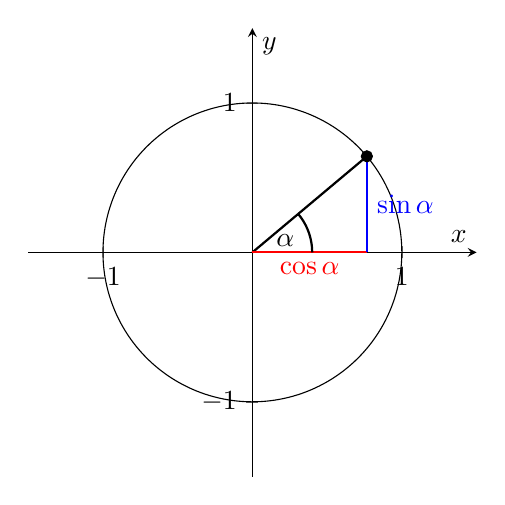
\begin{tikzpicture}
\begin{axis}[
    axis equal image,
    axis lines=middle,
    xmin=-1.5, xmax=1.5,
    ymin=-1.5, ymax=1.5,
    xtick={-1,0,1},
    ytick={-1,0,1},
    xlabel=$x$,
    ylabel=$y$
]

% Einheitskreis
\addplot[
  domain=0:360,
  samples=200
] ({cos(x)}, {sin(x)});

% Winkel in Grad
\def\winkel{40} 

% Punkt am Kreis
\addplot[mark=*] coordinates {({cos(\winkel)}, {sin(\winkel)})};

% Hypotenuse (schwarz)
\addplot[black, thick] coordinates {
  (0,0)
  ({cos(\winkel)}, {sin(\winkel)})
};

% Kosinus (rot, waagrecht)
\addplot[red, thick] coordinates {
  (0,0)
  ({cos(\winkel)},0)
} node[pos=0.5, below] {$\cos \alpha$};

% Sinus (blau, senkrecht)
\addplot[blue, thick] coordinates {
  ({cos(\winkel)},0)
  ({cos(\winkel)}, {sin(\winkel)})
} node[pos=0.5, right] {$\sin \alpha$};

% Winkel Alpha als Bogen
\addplot[domain=0:\winkel, samples=50, thick]	({0.4*cos(x)}, {0.4*sin(x)});

% Beschriftung Alpha
\node at (axis cs:0.22,0.08) {$\alpha$};

\end{axis}
\end{tikzpicture}
\end{center}
Da die Länge der Hypotenuse dem Radius des Kreises ($r=1$) entspricht, ist die Strecke der Ankathete von $\alpha$ gleich mit dem Kosinus. Ähnlich gilt für die Gegenkathete, dass sie gleich lang wie der $\sin \alpha$ ist. \par
Üblicherweise gibt man Winkel graphisch im Gradmaß mit Winkel $\alpha$ an, doch es gibt auch die Alternative mit dem \textbf{Bogenmaß}\index{Bogenmaß} $b$, für das gilt:
\[ b = \dfrac{\alpha \cdot 2 \pi}{ \ang{360}}\]
Daraus folgen insbesondere $\ang{360} \ \hat{=} \ 2\pi$ und $\ang{180} \ \hat{=} \ \pi$, deren Werte man sich merken sollte. Durch den Einheitskreis können wir die Winkel aber auf beliebig große Winkel erweitern, die wir im Bogenmaß als $x$-Werte einer Funktion interpretieren können.

\begin{definition}
Die Sinus- und Kosinus-Funktion sind trigonometrische Funktionen, die periodisch verlaufen.
\index{Funktion!Trigonometrische Funktionen} \index{Sinus} \index{Kosinus}
\begin{center}
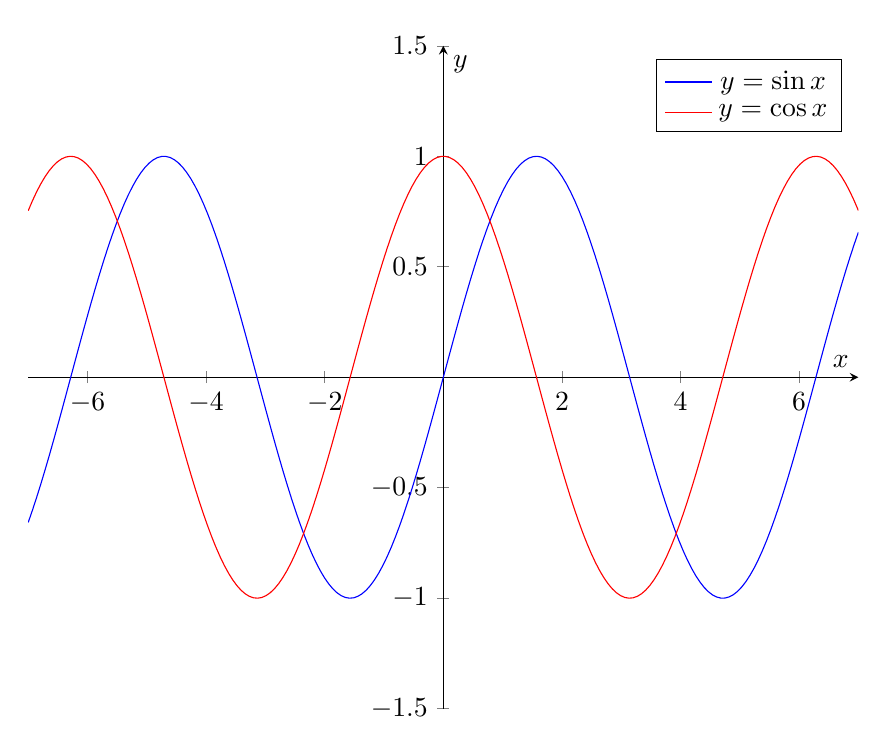
\begin{tikzpicture}
\begin{axis}[
    axis lines = middle,
    xlabel = $x$,
    ylabel = $y$,
    xmin=-7, xmax=7,
    ymin=-1.5, ymax=1.5,
    width=\textwidth,
    height=10cm,
]
\addplot[blue, domain=-7:7, samples = 200] {sin (deg(x))};
\addlegendentry{$y=\sin x$}
\addplot[red, domain=-7:7, samples = 200] {cos (deg(x))};
\addlegendentry{$y=\cos x$}
\end{axis}
\end{tikzpicture}
\end{center}

\end{definition}

Wir erkennen anhand des Graphen: Die Funktionen sind jeweils um $\frac{\pi}{2}$ zueinander verschoben. Wir fassen die wichtigsten Aussagen zusammen:
\begin{theorem} \textbf{(Eigenschaften der Sinus- und Kosinusfunktion)}
\begin{enumerate}
\item Der Definitionsbereich von $y=\sin x$ und $y=\cos x$ ist jeweils ganz $\R$,
\item Der Wertebereich ist ebenfalls identisch. Es gilt: $W_f = [-1;1]$.
\item Die Periode beider Funktionen ist $p=2\pi$.
\item Während $y=\sin x$ punktsymmetrisch zum Ursprung ist, ist $y=\cos x$ achsensymmetrisch zur $y$-Achse. 
\item Die Nullstellen der Sinusfunktion lauten für $k \in \Z$: $x_k=k \cdot z$. Für die Kosinusfunktion sind alle Nullstellen von der Form $x_k=\dfrac{\pi}{2}+k \cdot z$ darstellbar.
\item $\sin x = \cos \mleft( x-\dfrac{\pi}{2} \mright) \Leftrightarrow \cos x = \sin \mleft( x + \dfrac{\pi}{2}  \mright)$
\item Aus der Mittelstufe ist der \textit{trigonometrische Pythagoras}\index{Pythagoras!trigonometrischer} bekannt: Für alle $x\in \R$ gilt: $\sin^2 (x) + \cos^2 (x) = 1$. \footnote{Eine gute Übung ist es, diese Beziehung anhand des Einheitskreises herzuleiten.}
\end{enumerate}
\end{theorem}
Wichtig ist in diesem Zusammenhang auch nochmals Satz \ref{Periode_SinCos}, mit dem wir uns die Periode der beiden Funktionen im Allgemeinfall berechnen können.

\subsubsection{Exponentialfunktionen}
In vielen Anwendungen wie Abklings-, Wachstums- oder Zerfallsprozessen spielen Exponentialfunktionen eine zentrale Rolle. Mit ihnen kann man Sachzusammenhänge präzise modellieren und dadurch berechenbar machen. Zuerst wollen wir uns dafür nochmals die Rechenregeln der \textbf{Potenzen} in Erinnerung rufen, die wir für Exponentialfunktionen oft brauchen. 

\begin{theorem} \ \par
\begin{tabularx}{\textwidth}{X X}
\setstretch{2}
\textbf{Rechenregeln für Potenzen} & \textbf{Zahlenbeispiele} \\
\\
1.   $a^m\cdot a^n=a^{m+n}$ & $2^3\cdot 2^2=2^{3+2} = 2^5 = 32$ \\
\\
2.   $\dfrac{a^m}{a^n}=a^{m-n}$ & $\dfrac{3^5}{3^7}=3^{5-7}=3^{-2}=\dfrac{1}{3^2}=\dfrac{1}{9}$ \\
\\
3.   $(a^m)^n=a{m\cdot n}$ & $(2^3)^5=2^{3\cdot 5}=2^{15}=32768$
\index{Potenzen}
\end{tabularx}
\end{theorem}

\begin{definition} Für die Potenz $a^x, a>0$ heißt die in den reellen Zahlen definierte Funktion $f(x)=a^x$ \textbf{Exponentialfunktion}.
\label{Def:Expon}
\index{Exponentialfunktion} \index{Funktion!Exponential}
\end{definition}

\begin{theorem} \textbf{(Satz über Exponentialfunktionen)}
\begin{enumerate}[1.]
\item Die Wertemenge einer Exponentialfunktion $f$ ist stets $W_f=\R^+$. 
\item Für $0<a<1$ ist $f$ streng monoton fallend. Für $a>1$ steigt die Funktion streng monoton.
\end{enumerate}
\label{Satz_Exponentialfunktion}
\end{theorem}

\begin{example} \

\begin{enumerate}
\item Betrachten wir die Funktion $f(x)=\mleft( \dfrac{2}{3} \mright)^x$, so wissen wir nach Satz \ref{Satz_Exponentialfunktion}, dass $f(x)$ streng monoton fallend sein muss. Ein Abgleich mit dem Graphen bestätigt uns das.
\item Die Funktion $g(x)=2^x$ ist streng monoton steigend.
\end{enumerate}
\begin{center}
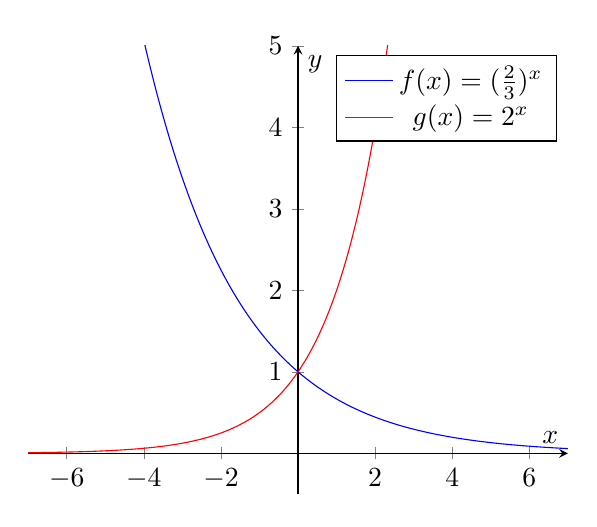
\begin{tikzpicture}
\begin{axis}[
    axis lines = middle,
    xlabel = $x$,
    ylabel = $y$,
    xmin=-7, xmax=7,
    ymin=-0.5, ymax=5,
   % width=\textwidth,
    %height=10cm,
]
\addplot[blue, domain=-7:7, samples = 200] {(2/3)^x};
\addlegendentry{$f(x)=\mleft( \frac{2}{3} \mright)^x$}
\addplot[red, domain=-7:7, samples = 200] {(2)^x};
\addlegendentry{$g(x)=2^x$}
\end{axis}
\end{tikzpicture}
\end{center}
\end{example}

Von besonderer Bedeutung ist die Exponentialfunktion 
\[ y=e^x \]
Dabei ist $e$ die \textit{Eulersche Zahl}, die durch den Grenzwert 
\[
e=\lim_{n\rightarrow \infty} \mleft( 1+\dfrac{1}{n}\mright) ^n = \num{2,718281}...
\]
definiert ist. Die Funktion $y=e^x$ nennen wir auch $e$-Funktion. Sie ist mit Abstand die wichtigste Exponentialfunktion. 
\begin{theorem} \
\begin{enumerate}
\item Jede Exponentialfunktion aus Definition \ref{Def:Expon} ist darstellbar als $f(x)=e^{\lambda\cdot x}$ mit $\lambda = \ln a$ (siehe Definition \ref{Def:Logarithmus}). 
\item Für $\lambda > 0$ ist die $e$-Funktion streng monoton steigend.
\item Ist $\lambda < 0$, so fällt die Funktion streng monoton. 
\end{enumerate}
\end{theorem}

\subsubsection{Logarithmusfunktionen}
\begin{definition}
Die Lösung der Exponentialgleichung $r=a^x$ mit $r\in \R^+, a>0$ und $x\in \R$ bezeichnet man als \textbf{Logarithmus} von $r$. Man schreibt:
\[ x=\log_a(r)  \]
Der spezielle Logarithmus zur Gleichung $b=e^x$ mit $b \in \R^+, x\in \R$ heißt \textbf{natürlicher Logarithmus} mit 
\[ x= \log_e(b) = \ln b \]
\label{Def:Logarithmus}
\index{Logarithmus} \index{Natürlicher Logarithmus}
\end{definition}

\begin{theorem} \ \par

\begin{tabularx}{\textwidth}{X X}
\setstretch{2}
\textbf{Rechenregeln für Logarithmen} & \textbf{Zahlenbeispiele} \\
\\
1.   $\log_a (u\cdot v) = \log_a u + \log_a v$ & $\log_2 (8\cdot 4) = \log_2 8 + \log_2 4 = 3+2=5$ \\
\\
2.   $\log_a\mleft( \dfrac{u}{v} \mright) = \log_a u - \log_a v$ & $\log_3\mleft( \dfrac{81}{27} \mright) = \log_3 81 - \log_3 27=4-3=1$ \\
\\
3.   $\log_a u^n = n \cdot \log_a u$ & $\log_5 125^4 = 4 \cdot \log_5 125=4\cdot 3 = 12$ \\
\\
4.   $\log_a a^x = x \cdot \underbrace{\log_a a}_1 = x$ & $\ln e^x = x \underbrace{\ln e}_1 = x$ \\
\\
5.   $a^{\log_a x} = x$ & $e^{\ln x} = x$ \\
\\
6.   $\ln f(x) = \ln g(x) \Rightarrow f(x) = g(x)$ 

\end{tabularx}
\end{theorem}

Nun gehen wir analog wie bei den Exponentialfunktion vor: Wir ersetzen $b$ mit $x$ und erhalten die natürliche Logarithmusfunktion:

\begin{definition}

Die Funktion $y=\ln x$ heißt natürliche Logarithmusfunktion. \index{Funktion!Logarithmusfunktion} \index{Logarithmusfunktion}

\end{definition}

\begin{theorem} \textbf{(Eigenschaften der natürlichen Logarithmusfunktion)} \par
Nehme $f(x)=\ln x$ und $g(x)=e^x$. Dann gilt:
\begin{enumerate}
\item Die Definitionsmenge von $y=\ln x$ ist gleich mit der Wertemenge von $y=e^x$, die jeweils zueinander die Umkehrfunktion darstellen. Es gilt also $D_f = W_g=\R^+$.
\item Daraus folgt direkt: $W_f=D_g=\R$
\item $f(x)$ hat eine Nullstelle bei $x=1$, da $\ln 1 = 0$ ist.
\item Die $\ln$-Funktion ist streng monoton steigend.
\end{enumerate}
\label{Satz:E-Logarithmus}
\end{theorem}

\begin{example}
Wir betrachten im Folgenden die natürliche Logarithmusfunktion $f(x)=\ln (2x^2-2)$. Wegen Satz \ref{Satz:E-Logarithmus} 1. müssen wir $2x^2+2>0$ setzen. Da das für alle reellen Zahlen gilt, ist $D_f=\R^+$. Die Wertemenge hängt von der Wertemenge von $h(x)=2x^2+2$ ab, denn jeder $y$-Wert unserer Hilfsfunktion $h$ ergibt einen $y$-Wert von $f$ selbst. Für $W_h$ gilt $y\geq 2$ (Übung). Unsere Werte, die wir in $\ln x$ einsetzen, sind genau die $y$-Werte von $h$, also ist der kleinste Wert für unsere Funktion $f$ selbst $\ln 2$. Jeder andere Wert ist größer, und damit ist die Wertemenge von $f$ genau $W_f=\{ y \in \R | y \geq \ln 2  \}$. Da $1 \notin W_h$ liegt, hat $f$ auch keine Nullstellen. \par
\textit{Hinweis:} Dieses Beispiel ist schon sehr anspruchsvoll. Die eigenständige Lösung wird in der Schule vermutlich nicht erwartet. Als eigene Übung könnte man aber die vier Aspekte aus Satz \ref{Satz:E-Logarithmus} auf die Funktion $y=\ln (2x)$ anwenden.
\end{example}

\subsubsection{Betragsfunktionen}

\begin{definition}
Sei $y=f(x)$ eine beliebige Funktion, so heißt die Funktion $|y|=f(x)$ \textbf{Betragsfunktion}, die jedem $x$ Wert den Betrag von $f(x)$ zuordnet:
\[ |f|: x \mapsto |f(x)|\]
\index{Funktion!Betragsfunktion} \index{Betragsfunktion}
\end{definition}

\begin{example}
Sei $f(x)=|x|$ unsere Betragsfunktion. So können wir sie ausdrücken als $f(x)=\begin{cases} x & \mathrm{für} x\geq 0 \\ -x & \mathrm{für} x<0
\end{cases}$. Den Graphen von $f$ ermittelt man, indem man den Graphen für $y=x$ zeichnet und alles unterhalb der $x$-Achse an der $x$-Achse spiegelt:

\begin{center}
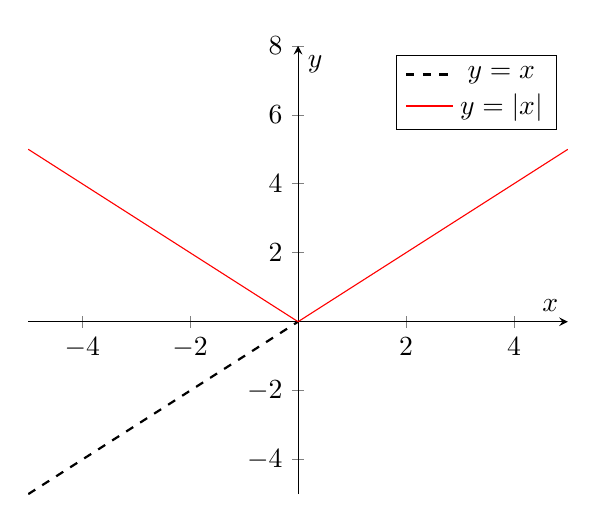
\begin{tikzpicture}
\begin{axis}[
    axis lines = middle,
    xlabel = $x$,
    ylabel = $y$,
    xmin=-5, xmax=5,
    ymin=-5, ymax=8,
   % width=\textwidth,
    %height=10cm,
]
\addplot[black, dashed, thick, domain=-5:0, samples = 200] {x};
\addlegendentry{$y=x$}
\addplot[red, domain=-5:0, samples = 200] {-x};
\addplot[red, domain=0:5, samples = 200] {x};
\addlegendentry{$y=|x|$}
\end{axis}
\end{tikzpicture}
\end{center}

\end{example}

Da wir uns nun mit Funktionen auskennen, können wir in ein zentrales Themengebiet der Analysis übergehen: die Differentialrechnung.

\newpage


\subsection{Grundlagen der Differentialrechnung}


\begin{definition} \textbf{(Über das Schneiden und Berühren zweier Graphen)} 
\begin{enumerate}
\item Die Graphen zweier Funktionen $f$ und $g$ schneiden\index{Funktion!Schneiden und Berühren} \index{Schneiden zweier Funktionen} sich in einem Punkt genau dann, wenn sie diesen Punkt gemeinsam haben.
\item Die Graphen zweier Funktionen $f$ und $g$ berühren\index{Funktion!Berühren} sich in einem Punkt genau dann, wenn sie diesen Punkt gemeinsam und dort die gleiche Steigung haben.
\item Eine Gerade, die einen Funktionsgraphen in einem Punkt berührt, heißt \textbf{Tangente}. \index{Tangente}
\item Eine Gerade, die einen Funktionsgraphen in mehreren Punkten schneidet, heißt \textbf{Sekante}. \index{Sekante}
\end{enumerate}
\end{definition} 

\begin{definition} \textbf{(Formale Grundbegriffe der Ableitung)}
\begin{enumerate}
\item Der Term $\dfrac{f(x)-f(x_0)}{x-x_0}$ heißt \textbf{Differenzenquotient}.
\item Der Grenzwert $\lim\limits_{x\to x_0} \dfrac{f(x)-f(x_0)}{x-x_0} = \lim\limits_{h \to 0} \dfrac{f(x_0+h)-f(x_0)}{h}$ heißt \textbf{Differentialquotient}.
\item Eine Funktion $f$ heißt an der Stelle $x_0$ differenzierbar, wenn der beidseitige Grenzwert des Differenzenquotienten existiert und gleich ist.
\item Für eine an der Stelle $x_0$ differenzierbare Funktion heißt der Differentialquotient \[ f'(x_0)=\lim_{x\to x_0} \dfrac{f(x)-f(x_0)}{x-x_0} = \lim_{h \to 0} \dfrac{f(x_0+h)-f(x_0)}{h} \] \textbf{Ableitung von $\mathbf{f}$ an der Stelle $\mathbf{x_0}$}.
\end{enumerate}
\index{Differentialquotient} \index{Funktion!Ableitung} \index{Ableitung}
\end{definition}

\begin{example}
Betrachten wir die Funktion $f(x)=x^2$ an der Stelle $x_0=1$. Den Differentialquotienten bestimmen wir wiefolgt:
\[ \lim_{h\to 0^+} =  \dfrac{f(x_0+h)-f(x_0)}{h} = \lim_{h\to 0^+} \dfrac{(1+h)^2-1^2}{h} = \lim_{h\to 0^+} \dfrac{2h+h^2}{h} =  \lim_{h\to 0^+} 2+h = 2\]
\[ \lim_{h\to 0^-} =  \dfrac{f(x_0+h)-f(x_0)}{h} = \lim_{h\to 0^-} \dfrac{(1+h)^2-1^2}{h} = \lim_{h\to 0^-} \dfrac{2h+h^2}{h} =  \lim_{h\to 0^-} 2+h =2\]
Da der Grenzwert existiert und beidseitig übereinstimmt ($2=2$ ist offensichtlich), heißt $f$ für $x_0 = 1$ differenzierbar mit Ableitung $f'(1)=2$. \par
Graphisch können wir die Abeltiung auch ermitteln. Sie ist die Steigung der Tangente, die den Graphen $G_f$ im Punkt $P(x_0|f(x_0))$ berührt. Wir sehen:
\begin{center}
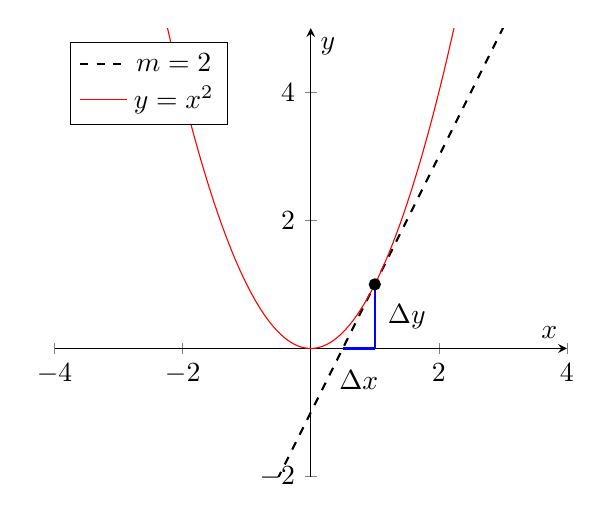
\begin{tikzpicture}
\begin{axis}[
    axis lines = middle,
    xlabel = $x$,
    ylabel = $y$,
    xmin=-4, xmax=4,
    ymin=-2, ymax=5,
    legend pos = north west,
    axis equal image
]

% Gerade y=x
\addplot[black, dashed, thick, domain=-4:4, samples=200] {2*x-1};
\addlegendentry{$m=2$}

% Parabel
\addplot[red, domain=-4:4, samples=200] {x^2};
\addlegendentry{$y=x^2$}

% Punkt (1,1)
\addplot[mark=*] coordinates {(1,1)};

% Steigungsdreieck für y = x
% horizontal
\addplot[blue, thick] coordinates {(1/2,0) (1,0)};
% vertikal
\addplot[blue, thick] coordinates {(1,0) (1,1)};
% Beschriftungen
\node at (axis cs:0.75,-0.5) {$\Delta x$};
\node at (axis cs:1.5,0.5) {$\Delta y$};

\end{axis}
\end{tikzpicture}
\end{center}
Durch das Ermiltten des Steigungsdreiecks ergibt sich $m=\dfrac{\Delta y}{\Delta x} = \dfrac{1}{\frac{1}{2}} = 2$
\end{example}

Im Folgenden ersetzen wir die Bezeichnung $f'(x_0)$ durch $f'(x)$ und meinen damit eine ganze Funktion, die Ableitungsfunktion:

\begin{definition} \textbf{(Ableitungsfunktion)} \par
Sei $f:D_f \rightarrow W_f, x \mapsto f(x)$ eine vollständig differenzierbare Funktion, so heißt die Funktion $f'(x)$ die \textbf{Ableitungsfunktion} von $f$, die jedem $x_0\in D_f$ die Steigung an der Stelle $x_0$ (Ableitung) zuordnet.
\end{definition}

\begin{theorem}\textbf{(Ableitungen ausgewählter Funktionen)} \par
\renewcommand{\arraystretch}{1.3}
\begin{tabularx}{\textwidth}{X | X}

\textbf{Funktion $f(x)$} & \textbf{Ableitung $f'(x)$} \\
\hline
Konstante Funktion \hfill $c=konst.$ & $0$ \\
\hline
Potenzfunktion \hfill $x^n$, $n\in\Q \setminus \{ 0 \}$ & $n\cdot x^{n-1}$ (Potenzregel) \\
\hline
Sinusfunktion \hfill $\sin x$ & $\cos x$ \\
\hline
Kosinusfunktion \hfill $\cos x$ & $-\sin x$ \\
\hline
Exponentialfunktion \hfill $a^x$ & $(\ln a)\cdot a^x$ \\
\hline
$e$-Funktion \hfill $e^x$ & $e^x$ \\
\hline
Logarithmusfunktion \hfill $\log_a x$ & $\frac{1}{(\ln a) x}$\\
\hline
$\ln$-Funktion \hfill $\ln x$ & $\frac{1}{x}$ \\
\end{tabularx}
\renewcommand{\arraystretch}{1}
\label{Satz:Ableitungen_Funktionen}
\end{theorem}

\subsubsection{Ableitungsregeln}
Wir fassen hier die wichtigsten Ableitungsregeln zusammen, und gehen anschließend auf einige Beispiele ein.

\begin{theorem} \textbf{(Ableitungsregeln)} \par
Sei $k\in \R \setminus \{ 0 \}$ eine Konstante und $u(x), v(x)$ zwei vollständig differenzierbare Funktionen. Dann gilt:
\begin{enumerate}
\item $f(x)= k \cdot u(x) \Rightarrow f'(x)=k \cdot u'(x)$ (Faktorregel)
\item $f(x)=u(x)+v(x) \Rightarrow f'(x)=u'(x)+v'(x)$ (Summenregel)
\item $f(x)=u(x) \cdot v(x) \Rightarrow f'(x)=u'(x)\cdot v(x) + u(x)\cdot v'(x)$ (Produktregel)
\item $f(x)=\dfrac{u(x)}{v(x)} \Rightarrow f'(x)=\dfrac{u'(x)\cdot v(x) - u(x) \cdot v'(x)}{\mleft( v(x) \mright)^2}$ (Quotientenregel)
\item $f(x)=u(v(x)) \Rightarrow f'(x)=u'(v(x))\cdot v'(x)$ (Kettenregel)
\end{enumerate}
\textit{Bemerkung:} Die Regeln 1, 2, 3 und 5 stehen in der Formelsammlung. Die Quotientenregel ist äußerst praktisch, deshalb lohnt es sich, diese auswendig zu lernen.
\label{Satz:Ableitungsregeln}
\index{Ableitungsregeln} \index{Funktion!Ableitungsregeln} \index{Produktregel} \index{Quotientenregel} \index{Kettenregel}
\end{theorem}
 
Um die Sätze \ref{Satz:Ableitungen_Funktionen} und \ref{Satz:Ableitungsregeln} zu üben, folgen hier einige Beispiele:

\begin{example} \
\begin{enumerate}
\item $y=4x^3+x^2+ \sin x \Rightarrow y' = 12x^2+2x+\cos x$
\item $y=\cos x + \sin x \Rightarrow y' = - \sin x + \cos x$
\item $y=4 \sin x \Rightarrow y'=4 (\sin x)'=4\cos x$
\item $y=(4x^3-3x)\cdot (2e^x-\sin x) \Rightarrow y'=(12x^2-3)(2e^x-\sin x)+(4x^3-3x)(2e^x-\cos x)$
\item $y=\dfrac{\ln x}{e^x} \Rightarrow y'=\dfrac{1-\ln x}{x\cdot e^x}$
\item $y=(3x-4)^{2026} \Rightarrow y'=2026 \cdot (3x-4)^{2025} \cdot 3 = 6078 (3x-4)^{2025}$
\end{enumerate}
\end{example}

\newpage

\subsection{Anwendung der Differentialrechnung}
\subsubsection{Bestimmung einer Tangente bzw. Normalen}
\begin{theorem}
Sei $f(x)$ eine vollständig differenzierbare Funktion. Dann erhalten wir die Tangentengleichung für einen Punkt $P(x_0|f(x_0))$ wiefolgt:

\begin{enumerate}
\item Bestimme den Term der Ableitung der Funktion $f(x)$.
\item Bestimme die Steigung an der Stelle $x_0$: $m=f'(x_0)$.
\item Bestimme den $y$-Wert $f(x_0)$. 
\item Setze alle Werte in die Tangentengleichung ein: $f(x_0)=f'(x_0) \cdot x_0 +t = m x_0 +t$
\item Bestimme zuletzt $t$ und gebe die vollständige Tangentengleichung an.
\end{enumerate}
Dieses Vorgehen ist analytisch und lässt sich leicht nachvollziehen. Eine andere Möglichkeit, die sich eher zum Auswendiglernen anbietet, und zu den oben genannten Schritten äquivalent ist, ist die Folgende: \par
\[ y=f'(x_0) \cdot (x-x_0)+f(x_0) \]
\label{Satz:Tangente}
\index{Tangente!Bestimmung der Tangentengleichung}
\end{theorem}

\begin{example}
Betrachten wir die Funktion $f(x)= x^3-4x+2$. Die Tangentengleichung für $x=2$ erhalten wir nach Methode \glqq unten\grqq \ durch
\[ y=f'(2) \cdot (x-2) + f(2) = 8 (x-2) + 2 = 8x -14  \]
Es ist eine gute Übung, die fünf Schritte durchzugehen, um die obere Rechnung nachzuvollziehen und die Tangente für $x=-1$ mit beiden Methoden zu bestimmen.
\label{Bsp:Tangente}
\end{example}

Neben der Tangente gibt es auch noch eine weitere Gerade, die manchmal eine Rolle spielt. Hierbei handelt es sich um die Normale.

\begin{definition}
Eine Gerade heißt Normale, wenn sie einen Graphen im $\ang{90}$-Winkel schneidet.
\end{definition}

\begin{theorem}
Sei $P(x_0|f(x_0))$ ein Punkt eines Graphen $G_f$ von einer vollständig differenzierbaren Funktion $f$, so ist die Gleichung
\[ y=\frac{-1}{f'(x_0)}\cdot (x-x_0) + f(x_0)\]
die Gleichung der Normalen durch den Punkt $P$.
\label{Satz:Normale}
\index{Normale}
\end{theorem}

\begin{example}
Greifen wir nochmals die Funktion aus Beispiel \ref{Bsp:Tangente} auf. Mithilfe der Formel aus Satz \ref{Satz:Normale} erhalten wir die Normalengleichung
\[ y=\dfrac{-1}{8}(x-2)+2  \]
Zusammen mit der Tangentengleichung erhalten wir folgendes Bild:
\begin{center}
\begin{tikzpicture}
\begin{axis}[
    axis lines = middle,
    xlabel = $x$,
    ylabel = $y$,
    xmin=-6, xmax=6,
    ymin=-3, ymax=6,
    legend pos = north west,
    axis equal image,
    width=\textwidth
]


%\addplot[black, dashed, thick, domain=-4:4, samples=200] {x^3-4*x+2};
%\addlegendentry{$m=2$}

% Parabel
\addplot[black, domain=-3:3, samples=200] {x^3-4*x+2};
\addlegendentry{$y=x^3-4x+2$}

%Tangente
\addplot[red, dashed, domain=-6:6, samples=200] {8*x-14};
\addlegendentry{Tangente}

%Normale
\addplot[blue, dashed, domain=-6:6, samples=200] {(-1/8)*x+2.25};
\addlegendentry{Normale}

% Punkt (2,2)
\addplot[mark=*] coordinates {(2,2)};

\end{axis}
\end{tikzpicture}
\end{center}
Hier bietet es sich an, die Schritte aus Satz \ref{Satz:Tangente} auf die Normale zu übertragen und zu überlegen, welche Schritte gleich, und welche unterschiedlich sind.
\end{example}

\subsubsection{Monotonie und Krümmungsverhalten}

Das Monotonie- und Krümmungsverhalten einer (zweimal differenzierbaren) Funktion $f(x)$ kann man im wesentlichen über die erste und zweite Ableitung $f'(x)$ und $f''(x)$ bestimmen.
\paragraph{Geometrische Bedeutung der ersten Ableitung} Die erste Ableitung repräsentiert anschaulich die Steigung des Graphen an der betrachteten Stelle. Für eine Stelle $x_0$ gilt nun:
\begin{itemize}
\item $f'(x_0)>0$: Der Funktionsgraph wächst \textit{streng monoton}.
\item $f'(x_0)=0$: Der Funktionsgraph hat die Steigung $0$ und verläuft an dieser Stelle flach.
\item $f'(x_0)<0$: Der Funktionsgraph fällt \textit{streng monoton}.
\end{itemize}
\paragraph{Geometrische Bedeutung der zweiten Ableitung} Die zweite Ableitung beschreibt \glqq die Steigung der Steigung\grqq. Viel anschaulicher ist aber die Formulierung, dass die zweite Ableitung die Änderung des Monotonieverhaltens ist, also angibt, wie viel sich die Steigung an der Stelle $x_0$ ändert. Man spricht hierbei auch vom \textbf{Krümmungsverhalten}. Es gilt:

\begin{itemize}
\item $f''(x_0)>0$: Die \textit{Steigung} des Graphen $G_f$ nimmt an der Stelle $x_0$ zu, d.h. die Tangente \textit{dreht sich im Uhrzeigersinn}. Der Graph $G_f$ besitzt daher an der Stelle $x_0$ eine \textbf{Linkskrümmung}.
\item $f''(x_0)<0$: Die \textit{Steigung} des Graphen $G_f$ nimmt an der Stelle $x_0$ ab, d.h. die Tangente \textit{dreht sich gegen den Uhrzeigersinn}. Der Graph $G_f$ besitzt daher an der Stelle $x_0$ eine \textbf{Rechtskrümmung}.
\end{itemize}
Wir fassen diese Erkenntnisse im nächsten Satz zusammen:

\begin{theorem}
Sei $f(x)$ eine zweimal differenzierbare Funktion. Betrachtet man die erste Ableitung $f'(x_0)$ an der Stelle $x_0$, so gilt:
\begin{itemize}
\item $f'(x_0)>0 \Rightarrow$ Die Funktion \textit{wächst} an der Stelle \textit{streng monoton}.
\item $f'(x_0)<0 \Rightarrow$ Die Funktion \textit{fällt} an der Stelle \textit{streng monoton}.
\item $f'(x_0)=0 \Rightarrow$ Die Funktion verläuft an der Stelle flach.
\end{itemize}
Für die zweite Ableitung $f''(x_0)$ gilt:
\begin{itemize}
\item $f''(x_0)>0 \Rightarrow$ Die Funktion ist an der Stelle \textit{linksgekrümmt}.
\item $f''(x_0)<0 \Rightarrow$ Die Funktion ist an der Stelle \textit{rechtsgekrümmt}.
\end{itemize}
\label{Satz:KrümmungMonotonie}
\index{Funktion!Krümmung}
\index{Funktion!Monotonie}
\index{Krümmungsverhalten einer Funktion}
\index{Monotonie einer Funktion}
\end{theorem}

\begin{example}
\item Betrachten wir zuerst die Normalparabel $y=x^2$. Für die erste Ableitung gilt: $y'=2x$. Deshalb können wir das Monotonieverhalten aufteilen in das Intervall $]-\infty, 0[$, indem die Funktion streng monoton fallend ist ($y'<0$). Für $x=0$ gilt $y'=0$, also ist hat die Normalparabel dort eine \glqq flache\grqq \ Stelle, an der der Graph waagrecht verläuft. Für $x>0$ ist die Normalparabel streng monoton steigend. Nun ermitteln wir die zweite Ableitung: $y''=2$. Deshalb ist die Normalparabel überall linksgekrümmt.
\begin{center}
\begin{tikzpicture}
\begin{axis}[
    axis lines = middle,
    xlabel = $x$,
    ylabel = $y$,
    xmin=-5, xmax=5,
    ymin=-2, ymax=5,
    legend pos = north west,
    axis equal image,
    width=\textwidth
]


%\addplot[black, dashed, thick, domain=-4:4, samples=200] {x^3-4*x+2};
%\addlegendentry{$m=2$}

% Parabel
\addplot[blue, domain=-3:3, samples=200] {x^2};
\addlegendentry{$y=x^2$}

% 1. Ableitung
\addplot[red, domain=-3:3, samples=200] {2*x};
\addlegendentry{$y'=2x$}

% 2. Ableitung
\addplot[black, domain=-5:5, samples=200] {2};
\addlegendentry{$y''=2$}

\end{axis}
\end{tikzpicture}
\end{center}
\label{Bsp:Monotonie}
\end{example}

\subsubsection{Extrem- Wende- und Terassenpunkte}

\begin{definition} \textbf{(Extrem-, Wende- und Terassenpunkte)} \par
Sei $f(x)$ eine dreifach differenzierbare Funktion. Dann heißt für
\begin{enumerate}
\index{Extrempunkt}
\item $f'(x_0)=0, f''(x_0)> 0$ der Punkt $P(x_0|f(x_0)$ \textbf{Tiefpunkt}, \index{Tiefpunkt}
\item $f'(x_0)=0, f''(x_0)< 0$ der Punkt $P(x_0|f(x_0)$ \textbf{Hochpunkt}, \index{Hochpunkt}
\item $f'(x_0)=0, f''(x_0)= 0, f'''(x_0)\neq 0$ der Punkt $P(x_0|f(x_0)$ \textbf{Terassenpunkt} oder Sattelpunkt, \index{Terassenpunkt} \index{Sattelpunkt}
\item $f''(x_0)= 0, f'''(x_0)\neq 0$ der Punkt $P(x_0|f(x_0)$ \textbf{Wendepunkt}. \index{Wendepunkt}
\end{enumerate}
Tief- und Hochpunkte werden oft auch gemeinsam als \textbf{Extrempunkte} bezeichnet, nimmt man Terassenpunkte hinzu, so spricht man von \textbf{kritischen Punkten}.
\label{Def:Extrempunkte}
\end{definition}
Aus der Definition ergibt sich unmittelbar, dass jeder Terassenpunkt ein Wendepunkt, aber nicht jeder Wendepunkt ein Terassenpunkt ist. Bei Terassen- und insbesondere Wendepunkten wird häufig noch danach gefragt, ob von links- nach rechtsgekrümmt oder der Graph andersherum sein Krümmungsverhalten ändert. \par
Betrachte nun erneut Beispiel \ref{Bsp:Monotonie}, und versuche, die \glqq flache Stelle\grqq \ mithilfe der Fachsprache aus der Definition \ref{Def:Extrempunkte} genauer zu beschreiben. Ein anderes Beispiel liefert vielleicht noch mehr Klarheit:

\begin{example} \
\begin{enumerate}
\item Sei $f(x)=\frac{1}{3}x^3-4x$ die betrachtete Funktion und unsere Aufgabe, die Wende- und Extrempunkte zu bestimmen. Zuerst bestimmen wir dafür die ersten drei Ableitungen:
\[ f'(x)=x^2-4,\hspace{1cm} f''(x)=2x, \hspace{1cm} f'''(x)=2\]
Für Extrempunkte gilt es, die Nullstellen der ersten Ableitung herauszufinden. Diese liegen bei $x_0=\pm 2$. Weil für $f''(x_0) = \pm 4 \neq 0$ gilt, liegen hier jeweils Extrempunkte vor. Für $x_0=-2$ ist die zweite Ableitung negativ. Also hat $f$ hier einen Hochpunkt. Analog gilt, dass $f$ bei $x_0=+2$ einen Tiefpunkt hat. Für den Wendepunkt bestimmen wir die Nullstellen der zweiten Ableitung und erhalten $x_W=0$. Da die dritte Ableitung für diesen $x$-Wert positiv ist, handelt es sich um einen Übergang von rechtsgekrümmt nach linksgekrümmt. Mithilfe der Funktionswerte geben wir nun die wirklichen Punkte an: \\
\[ H(-2|f(-2)) = (-2|\frac{16}{3}) \hspace{1cm} T(2|f(2)) = (2|\frac{-16}{3}) \hspace{1cm} W(0|f(0)) = (0|0)  \]
\begin{center}
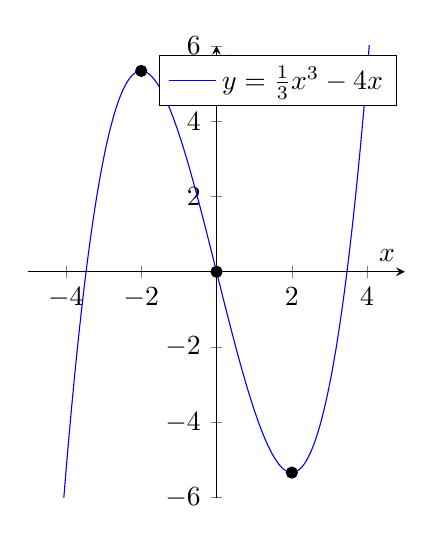
\begin{tikzpicture}
\begin{axis}[
    axis lines = middle,
    xlabel = $x$,
    ylabel = $y$,
    xmin=-5, xmax=5,
    ymin=-6, ymax=6,
    %legend pos = north west,
    axis equal image,
    width=0.7\textwidth
]


%\addplot[black, dashed, thick, domain=-4:4, samples=200] {x^3-4*x+2};
%\addlegendentry{$m=2$}

% Parabel
\addplot[blue, domain=-5:5, samples=200] {(1/3)*x^3-4*x};
\addlegendentry{$y=\frac{1}{3}x^3-4x$}

\addplot[mark=*] coordinates {(0,0)};
\addplot[mark=*] coordinates {(-2,16/3)};
\addplot[mark=*] coordinates {(2,-16/3)};

\end{axis}
\end{tikzpicture}
\end{center}
\item Durch Nachrechnen findet man heraus, dass die Funktion $y=(x-3)^3+5$ bei $T(3|5)$ einen Terassenpunkt hat. (Übung)
\end{enumerate}
\end{example}

\subsubsection{Zusammenfassung bis hierhin: Kurvendiskussion}
Aufbauend auf den vorherigen Kapiteln können wir nun intensive Betrachtungen für Funktionen und deren Verlauf anstellen. Bei dem Begriff \textit{Kurvendiskussion} geht es um die \textit{Untersuchung und Feststellung der Funktionseigenschaften und des Funktionsverlaufs}. Es gibt dabei kein konkretes Schema, aber häufig sind die folgenden Aspekte gefordert. Deshalb empfehle ich, diese Aspekte gut zu üben, um eine gute Prüfungsvorbereitung zu gewährleisten.
\begin{itemize}
\item Bestimmung des Definitionsbereiches (Definitionslücken)
\item Symmetrie (Punktsymmetrisch? Achsensymmetrisch?)
\item Null\textbf{stellen}, Schnitt\textbf{punkte} mit der $y$-Achse
\item (Senkrechte) Asymptoten
\item Ableitungen (i.d.R. bis zur dritten Ableitung)
\item Bestimmung der Extremwerte (Minima, Maxima)
\item Wendepunkte, Sattelpunkte
\item Verhalten der Funktion für $x\rightarrow \pm \infty$, Asymptoten im Unendlichen (waagrecht oder schräg)
\item Wertemenge der Funktion
\item Zeichnen der Funktion (sowie der Ableitung, und der Stammfunktion)
\item Untersuchung des Krümmungsverhaltens
\item Monotonie
\end{itemize}


\subsubsection{Extremwertaufgaben}
Ein etwas anderes Aufgabengebiet, und auch nicht wirklich der Analysis zuzurechnen, stellt der Bereich der Extremwertaufgaben da. Denn eigentlich geht es nicht, wie sonst bei der Analysis, um Funktionen, sondern um Gleichungen, die wir auflösen. Jedoch können wir mit unserem Wissen dieses Aufgabenformat, das wir seit der Mittelstufe kennen, etwas einfacher bearbeiten. \par
Zuerst stellt man in solchen Aufgabenformaten typischerweise die \textbf{Hauptbedingung} auf, eine Funktionsgleichung, die als Ergebnis die zu optimierende Größe liefert. Dabei kommt meist mehr als eine Variable vor. Anschließend stellt man eine Beziehung (die \textbf{Nebenbedingung}) zwischen Variablen auf und stellt diese Beziehung nach einer beliebigen Variable um. Bei drei Variablen sind zwei Nebenbedingungen erforderlich, usw. Hat man keine Idee, woraus man die Nebenbedingung(en) erstellen kann, so schaut man nochmal in der Aufgabenstellung nach mit der Frage im Kopf, welche Bedingung man noch nicht genutzt hat. Nun wird die Neben- in die Hauptbedingung eingesetzt. Dabei erhält man eine Funktion mit nur einer Variablen. Nun kann man die Funktion nach der Variablen ableiten und die Untersuchung als Extremwert-Problem betrachten (also Extrempunkte bestimmen). Die restlichen Größen werden laut Aufgabenstellung bestimmt. (\textit{Achtung: In der Praxis werden hier gerne Punkte liegengelassen, weil man diesen Aufgabenteil übersieht.}) Wir fassen diese Schritte im nächsten Satz zusammen:
\begin{theorem}\textbf{(Lösen von Extremwertaufgaben)}
\begin{enumerate}
\item Stelle eine Funktionsgleichung auf, die als Ergebnis die zu optimierende Größe liefert. \textbf{(Hauptbedingung)}
\item Stelle Beziehungen zwischen den Variablen auf. \textbf{(Nebenbedingungen)}
\item Setze die Nebenbedingungen in die Hauptbedingung ein.
\item Ermittle den gesuchten Extremwert (Hoch- oder Tiefpunkt).
\item Bestimme die restlichen Größen.
\end{enumerate}
\label{Satz:Extremwertaufgaben}
\index{Extremwertaufgaben}
\end{theorem}

\begin{example}
Ein Schäfer will mit $\SI{100}{\meter}$ Maschendraht für einen Zaun ein rechteckiges Feld für seine Schafe begrenzen, sodass die Fläche darin möglichst groß wird. Welche Länge $l$ und Breite $b$ muss das Rechteck erhalten?\par
Wir befolgen das Lösungsschema aus Satz \ref{Satz:Extremwertaufgaben}:
\begin{enumerate}
\item Die zu optimierende Größe ist der Flächeninhalt. Für ein Rechteck gilt: 
\[ A=l\cdot b \]
\item Die Gesamtlänge des Zaunes entspricht dem Umfang. Für ihn gilt:
\[ 2l + 2b = \SI{100}{\meter}	\Leftrightarrow 2l = \SI{100}{\meter} - 2b \Leftrightarrow l = \SI{50}{\meter}	- b \]
\item Wir setzen die Nebenbedingung in die Hauptbedingung ein: 
\[ A= (\SI{50}{\meter} -b)\cdot b =  \SI{50}{\meter} \cdot b - b^2 \]
\item Wir wollen den \textit{maximalen} Flächeninhalt bestimmen, suchen also den Hochpunkt der Funktion, die den Flächeninhalt beschreibt.
\[ A(b)=  \SI{50}{\meter} \cdot b - b^2\]
\[ A'(b)= \SI{50}{\meter} - 2b \]
\[ 0 = \SI{50}{\meter} - 2b_E \]
\[ 2b_E = \SI{50}{\meter} \Rightarrow b_E = \SI{25}{\meter} \]
wobei $b_E$ der Wert für den Extrempunkt darstellt. Um sicher zu gehen, prüfen wir, ob es sich dabei tatsächlich um einen Extrempunkt handelt. Dafür muss die zweite Ableitung an dieser Stelle kleiner $0$ sein. Tatsächlich gilt $A''(25)=-2 < 0$. (Übung)
\item Nachdem wir die Breite bestimmt haben, suchen wir noch die Länge des Rechteckes. Indem wir in die Nebenbedingung aus Schritt 2. einsetzen erhalten wir: $l_E=\SI{25}{\meter}$. 
\end{enumerate}
Oft ist ein Abschlusssatz schön. Deshalb schließen wir die Aufgabe mit den Folgenden Worten: \par
Der Schäfer sollte ein Quadrat der Seitenlänge $\SI{25}{\meter}$ wählen, um den größtmöglichen Flächeninhalt mit den $\SI{100}{\meter}$ Zaun zu erhalten.
\end{example}

\newpage

\subsection{Integralrechnung}
Im Unterricht haben wir Integrale als gemeinsamen Grenzwert von Ober- und Untersummen kennengelernt. Auf eine Wiederholung davon gehe ich an dieser Stelle nicht mehr ein, denn diese Vorüberlegung ist für den weiteren Verlauf aus meiner Sicht zu unwichtig, um ausführlich behandelt zu werden. Es lohnt sich aber dennoch, falls man genügend Zeit und Motivation hat, diese Einführung nochmals anzusehen! \par
Im Schulbuch wird an dieser Stelle aber noch die Summenschreibweise wiederholt, die ich hier deshalb auch nochmal anreißen möchte:
\[ \sum_{i=1}^n s_i = s_1 + s_2 + s_3 + ... + s_{n-1} + s_n  \]

\begin{definition}
Sei $f$ eine integrierbare Funktion, dann heißt jede Funktion $F(x)$ \textbf{Stammfunktion} von $f$, wenn gilt:
\[ F'(x)=f(x) \]
\index{Stammfunktion} \index{Funktion!Stammfunktion}
\end{definition}

\begin{example}
Gegeben ist die Funktion $f(x)=4x^3-8x$, so ist jede Funktion $F_c(x)=x^4-4x^2+c$ mit $c\in \R$ eine Stammfunktion, da die Ableitung der Funktion $F$ wieder $f$ ergibt. (Übung)
\begin{center}
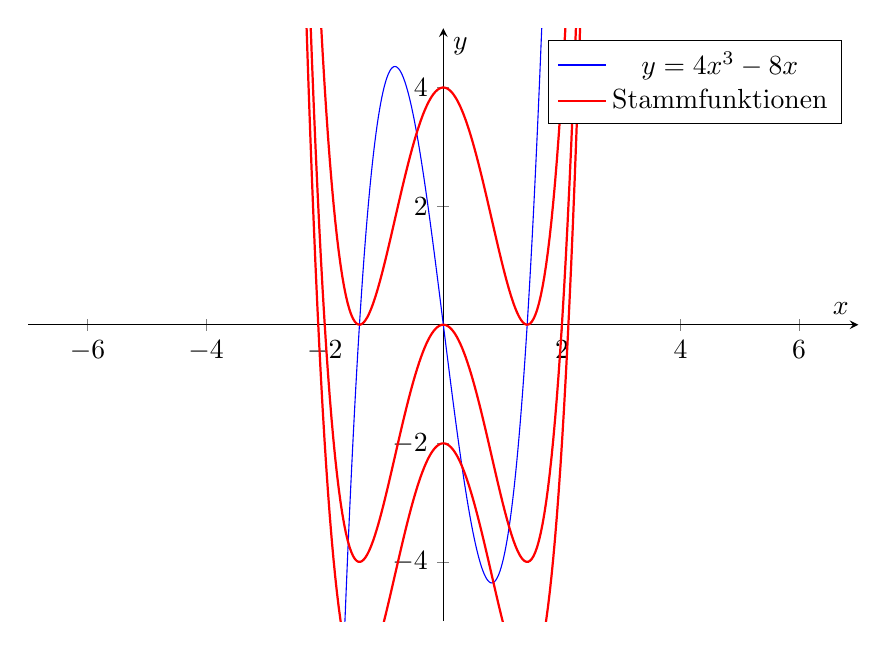
\begin{tikzpicture}
\begin{axis}[
    axis lines = middle,
    xlabel = $x$,
    ylabel = $y$,
    xmin=-7, xmax=7,
    ymin=-5, ymax=5,
    %legend pos = north west,
    axis equal image,
    width=\textwidth
]



% Parabel
\addplot[blue, domain=-2:2, samples=200] {4*x^3 - 8*x};
\addlegendentry{$y=4x^3-8x$}

\addplot[red, thick, domain=-3:3, samples=200] {x^4-4*x^2+4};
\addplot[red, thick, domain=-3:3, samples=200] {x^4-4*x^2};
\addplot[red, thick, domain=-3:3, samples=200] {x^4-4*x^2-2};
\addlegendentry{Stammfunktionen}

\end{axis}
\end{tikzpicture}
\end{center}


\end{example}
\subsubsection{Das bestimmte Integral}

\begin{definition} \textbf{(Bestimmtes Integral)} \par
Eine Funktion sei in einem Intervall $[a,b]$ definiert. Existiert der gemeinsame Grenzwert 
\[ \lim_{n\rightarrow +\infty} U_n = \lim_{n\rightarrow +\infty} O_n\] 
von Ober- und Untersumme im Intervall $[a,b]$, so nennt man diesen Grenzwert \textbf{bestimmtes Integral der Funktion $\mathbf{f}$} über $[a,b]$ und schreibt 
\[ \int_a^b f(x) \diff x  \]
Die Funktion $f$ nennt man dann \textbf{integrierbar} über $[a,b]$. Dabei heißt $f$ \textbf{Integrand} und die durch $\diff x$ gekennzeichnete Variable \textbf{Integrationsvariable}.
\index{Integral!Bestimmtes}
\index{Bestimmtes Integral}
\index{Integrand}
\end{definition}

\begin{theorem} \textbf{(Rechenregeln für das bestimmte Integral)} \par
\begin{enumerate}
\item $ \displaystyle \int_a^a f(x) \diff x = 0 $  
\item $\displaystyle \int_a^b f(x) \diff x + \int_b^c f(x) \diff x= \int_a^c f(x) \diff x $
\item $\displaystyle \int_b^a f(x) \diff x = -\int_a^b f(x) \diff x$
\end{enumerate}
\label{Satz:Rechenregeln_besIntegral}
\end{theorem}
Auf Beispiele wird an dieser Stelle verzichtet, die Rechenregeln werden in den folgenden Kapiteln aber Verwendung finden. \par
Im Abitur kann bzw. muss auch ohne Rechnung der Wert eines bestimmten Integrals ermittelt werden können. Es gibt dafür keine Allzweck-Methode, dennoch gibt es einige Ideen, mit denen man so eine Aufgabe bewältigen kann. 
\begin{enumerate}
\item \textbf{Kästchen zählen:} Das ist wohl die elementarste Variante. Zähle alle Kästchen unter dem Graphen bis zur $x$-Achse. Beachte immer den Maßstab: Wie groß ist ein Kästchen?
\item  \textbf{Geometrische Figuren:} Falls der Graph der Funktion gut liegt, kann es manchmal hilfreich sein, eine geometrische Figur, etwa ein Dreieck, Trapez, etc. in das Koordinatensystem zu zeichnen, das den Flächeninhalt möglichst gut approximiert (annähert). Die Formeln für diese elementargeometrischen Figuren sind Grundwissen und stehen zum Beispiel in der Formelsammlung. Für den hilfsmittelfreien Teil im Abitur ist es dennoch eine Überlegung wert, sich die Formeln auswendig zu merken.
\item Hast du weitere Ideen? Kreativ denken kann dir manchmal viel Zeit sparen. Wenn du also noch andere Ideen hast, ist das sehr gut!
\end{enumerate}

\begin{theorem}
Gegeben ist die auf dem Intervall $[a,b]$ integrierbare Funktion. Dann gibt das Integral $\displaystyle \int_a^b f(x) \diff x$ die \textbf{orientierte Flächenbilanz} der Fläche an, die der Graph von $f$ mit der $x$-Achse zwischen der unteren Grenze $a$ und der oberen Grenze $b$ einschließt. Dabei werden Flächeninhalte oberhalb der $x$-Achse positiv, darunterliegend negativ, gezählt.
\index{Flächenbilanz}
\end{theorem}


\newpage
% Index soll Stichwortverzeichnis heissen
\renewcommand{\indexname}{Stichwortverzeichnis}

% Stichwortverzeichnis soll im Inhaltsverzeichnis auftauchen
\addcontentsline{toc}{section}{Stichwortverzeichnis}

% Stichwortverzeichnis endgueltig anzeigen
\printindex
\end{document}

\begin{definition}

\end{definition}
